% -----------------------------------------------------------------------------
% 1) Introduce toy percolation model
% 2) Include stochastic infectivity parameter
% 3) Show behaviour in one and two dimensions
% 4) Set the basis model and establish the main ensemble method 
% -----------------------------------------------------------------------------

\chapter{Tree disease: a simple lattice model}
\label{chapter:SLM}

Typically, models of tree disease are complicated and involve multiple parameters informed by experimental data. Moreover, modelling a specific pathosystem requires in-depth, specialist knowledge to incorporate biological realism, such as pathogen lifecycles or environmental suitability. This introductory Chapter outlines a simple model of tree disease spreading through a forest that will lay the foundations for more detailed treatment in later Chapters.
Consequently, the compartmentalised $SIR$, percolation-based, model used by \cite{OROZCOFUENTES201912} will be re-examined. 

From first principles, the percolation model is analysed over a single tree density parameter ($\rho$), leading to a mathematical and conceptual definition of percolation in the context of tree-based epidemics. 
Then, a discussion of critical phenomena, universal behaviour, and self-similarity in the system will follow. Crucially, this Chapter demonstrates the importance of thresholds in the spread of tree-based diseases.

Having established a simple one-parameter model, a more involved two-parameter `stochastic percolation' model will be developed and examined. 
Stochastic percolation will include an extra parameter representing the degree of pathogen infectivity. 
In general, measuring infectivity is challenging and subject to much spatial and temporal variation, such as changing climatic/environment conditions or species-level genetic variations in susceptibilities.  
However, including a stochastic infectivity parameter is essential to construct representative models of tree-based epidemics, as infectivity (or susceptibility) can vary widely over a landscape.
The two-parameter model will constitute a simple lattice model (SLM) of disease dynamics. 
This introductory Chapter will introduce ensemble-averaging parameter sweeps, used throughout the thesis to categorize the SLM behaviour.

\section{Percolation formalism}
\label{sec:perc-form}
% understand universality class and scaling exponents 
% we consider small timescales and neglect regrowth factors
Consider a square lattice of size $L \times L$ , where each site in the lattice can be in one of two states: %
open with probability $\rho$ or closed with probability ($1-\rho$). %
Therefore, the probability $\rho$ describes a density parameter and encapsulates the occupancy of a homogeneous distribution of open and closed lattice positions.
One open site ($c_p$) is connected to another ($c_q$) if laid within the Von Neumann neighbourhood \cite{toffoli1987cellular}.

A connected set of open nearest neighbours define a cluster denoted by $C$, where $c_i \in C$.
Given the set $C$, it is possible to traverse between member sites $c_i \in C$ by moving through the lattice in either horizontal or vertical steps `Von Neumann motion'. 
Given two distinct non-overlapping clusters $c_i \in C_1$ and $c_j \in C_2$, then $c_i \neq c_j $ i.e. there is no way to jump from $C_1$ to $C_2$ following Von Neumann motion. 
Connectivity is defined between lattice sites rather than the edges which connect them, known as `site' percolation\textemdash as opposed to `bond' percolation.

If $\rho$ is close to zero, only small clusters would be present as a disordered system; 
conversely, if $\rho$ is large, a connected network of open positions would dominate the domain, thus defining an ordered system.
At some point for $\rho \in [0, 1]$, a critical threshold ($\rho_c$) would be reached and a singularity of connected sites would span an infinite sized lattice.
On a finite lattice, the cluster is said to percolate and form a `spanning cluster' ($C_\infty$) that extends between at least two different edges of the lattice.
The formation of the spanning cluster occurs abruptly between a very narrow range of $\rho$ values. 
Therefore, the threshold for percolation defines a critical-point \cite{STAUFFER19791}. 

The critical point can be defined as the least value of $\rho$ where percolation occurs with non-zero probability. %
This can be formalised by first considering the probability function: $\theta (\rho)= \lbrace \rho:|C|=\infty\rbrace$ where $\theta(\rho)$ is the probability of an arbitrary site, %
within a lattice of density $\rho$, belonging to cluster $C$ of size $\infty$ (i.e. the spanning cluster). %
The critical value then satisfies: %
\begin{equation}
\label{eq:critical_threshold_1d}
    \rho _{c}=sup \lbrace \rho : \theta (\rho ) = 0 \rbrace
\end{equation}
At this point, the spanning cluster has been described conceptually, although many nuances and technicalities complicate the definition. %
For example, the probability of percolation has a non-trivial dependence on the size of the lattice;
if the mean cluster size, defined by a `characteristic' cluster length $C_r$, is above or comparable to $L$, 
percolation could occur despite the density residing in the sub-critical regime. %
The size of the lattice is therefore required to be sufficiently large compared to individual lattice positions (or microscopic interactions) 
in order to approximate the threshold ($\rho_c$) reliably and produce a spanning cluster ($C_{\infty}$). 

When the domain size is large, the threshold $\rho_c$ will remains approximately constant and insensitive to small changes in the domain. 
All proceeding simulations in this Chapter are conducted on finite-sized domains between two and three orders of magnitude larger than individual lattice points.
The model presented in this Chapter (first published by \cite{OROZCOFUENTES201912}) was 
found to agree with the accepted percolation threshold, when the lattice had size $L \sim 500\times500$;
the lattice configuration used here will therefore assume the same size configuration. 

Intuitively, it is clear to see the link between percolation and epidemiology: 
open lattice positions act as susceptible members of a population ($S$), and $\rho$ defines a density of the hosts. 
In this paradigm, the spanning cluster describes a high-impact epidemic that spreads uncontrollably. 
Small to medium-sized clusters existing at (or slightly below) the threshold describe short-lived, 
failed epidemics where the pathogen spreads for a time before becoming extinct.

These analogies have clear limitations when describing mobile hosts, but fortunately, trees are sessile and immobile.
Thus, percolation theory provides a valuable framework for modelling tree diseases (see Chapter \ref{section:lit-rev-perc} 
for a review of percolation-based models). 
Forming a percolation-based lattice model of tree disease requires us first to combine a compartmental $SIR$-like model within the lattice ($L$) mentioned above. %
Next, an appropriate transmission dynamic is described to model the spread of disease between lattice points.


\section{Percolation-based $SIR$}

The percolation density parameter ($\rho$) defines a simple host distribution.
Namely, $\rho$ represents the probability of a susceptible tree $S$ (given a numerical value $1$), 
while empty lattice positions define an insusceptible state $\emptyset$ (with numerical value $0$).
If a susceptible tree neighbours an infected tree, it will transition into the $I$ compartment (having a numerical value of $2$).
Transitions between states occur with a probability of 1, and the Von-Neumann neighbourhood describes the connectivity between trees.
After an arbitrary number of time-steps $T$, an infected tree will transition into the removed state $R$ and die; 
see appendix \ref{a:propagation} for more information on the numerical implementation. %
For simplicity, the infectious lifetime will not be considered as a parameter but will remain fixed at $T=1.0$\textemdash revisited below in section \ref{ch3:two-param-model}.

The initial conditions begin with a small patch of infected hosts (of size $5\times5$) located at the origin ($L_O$) at $t=0$, and percolation events describe the boundary conditions. 
Percolation occurs when the infection spreads from $L_O$ to any of the four lattice boundaries;  thus defining a connected cluster of infectious-removed that spans the domain from $L_O$.
Each time-step through the simulation represents an arbitrary unit of time, and simulation termination occurs on one of three boundary conditions: 
1) a percolation is observed 
2) the pathogen becomes extinction 
3) a time-horizon of $N$ steps is reached. 
Typical simulations on a domain of size $500 \times 500$ are shown in Figure \ref{fig:ch3-perc-spread} through three time-steps. 

\begin{figure}
    \centering
    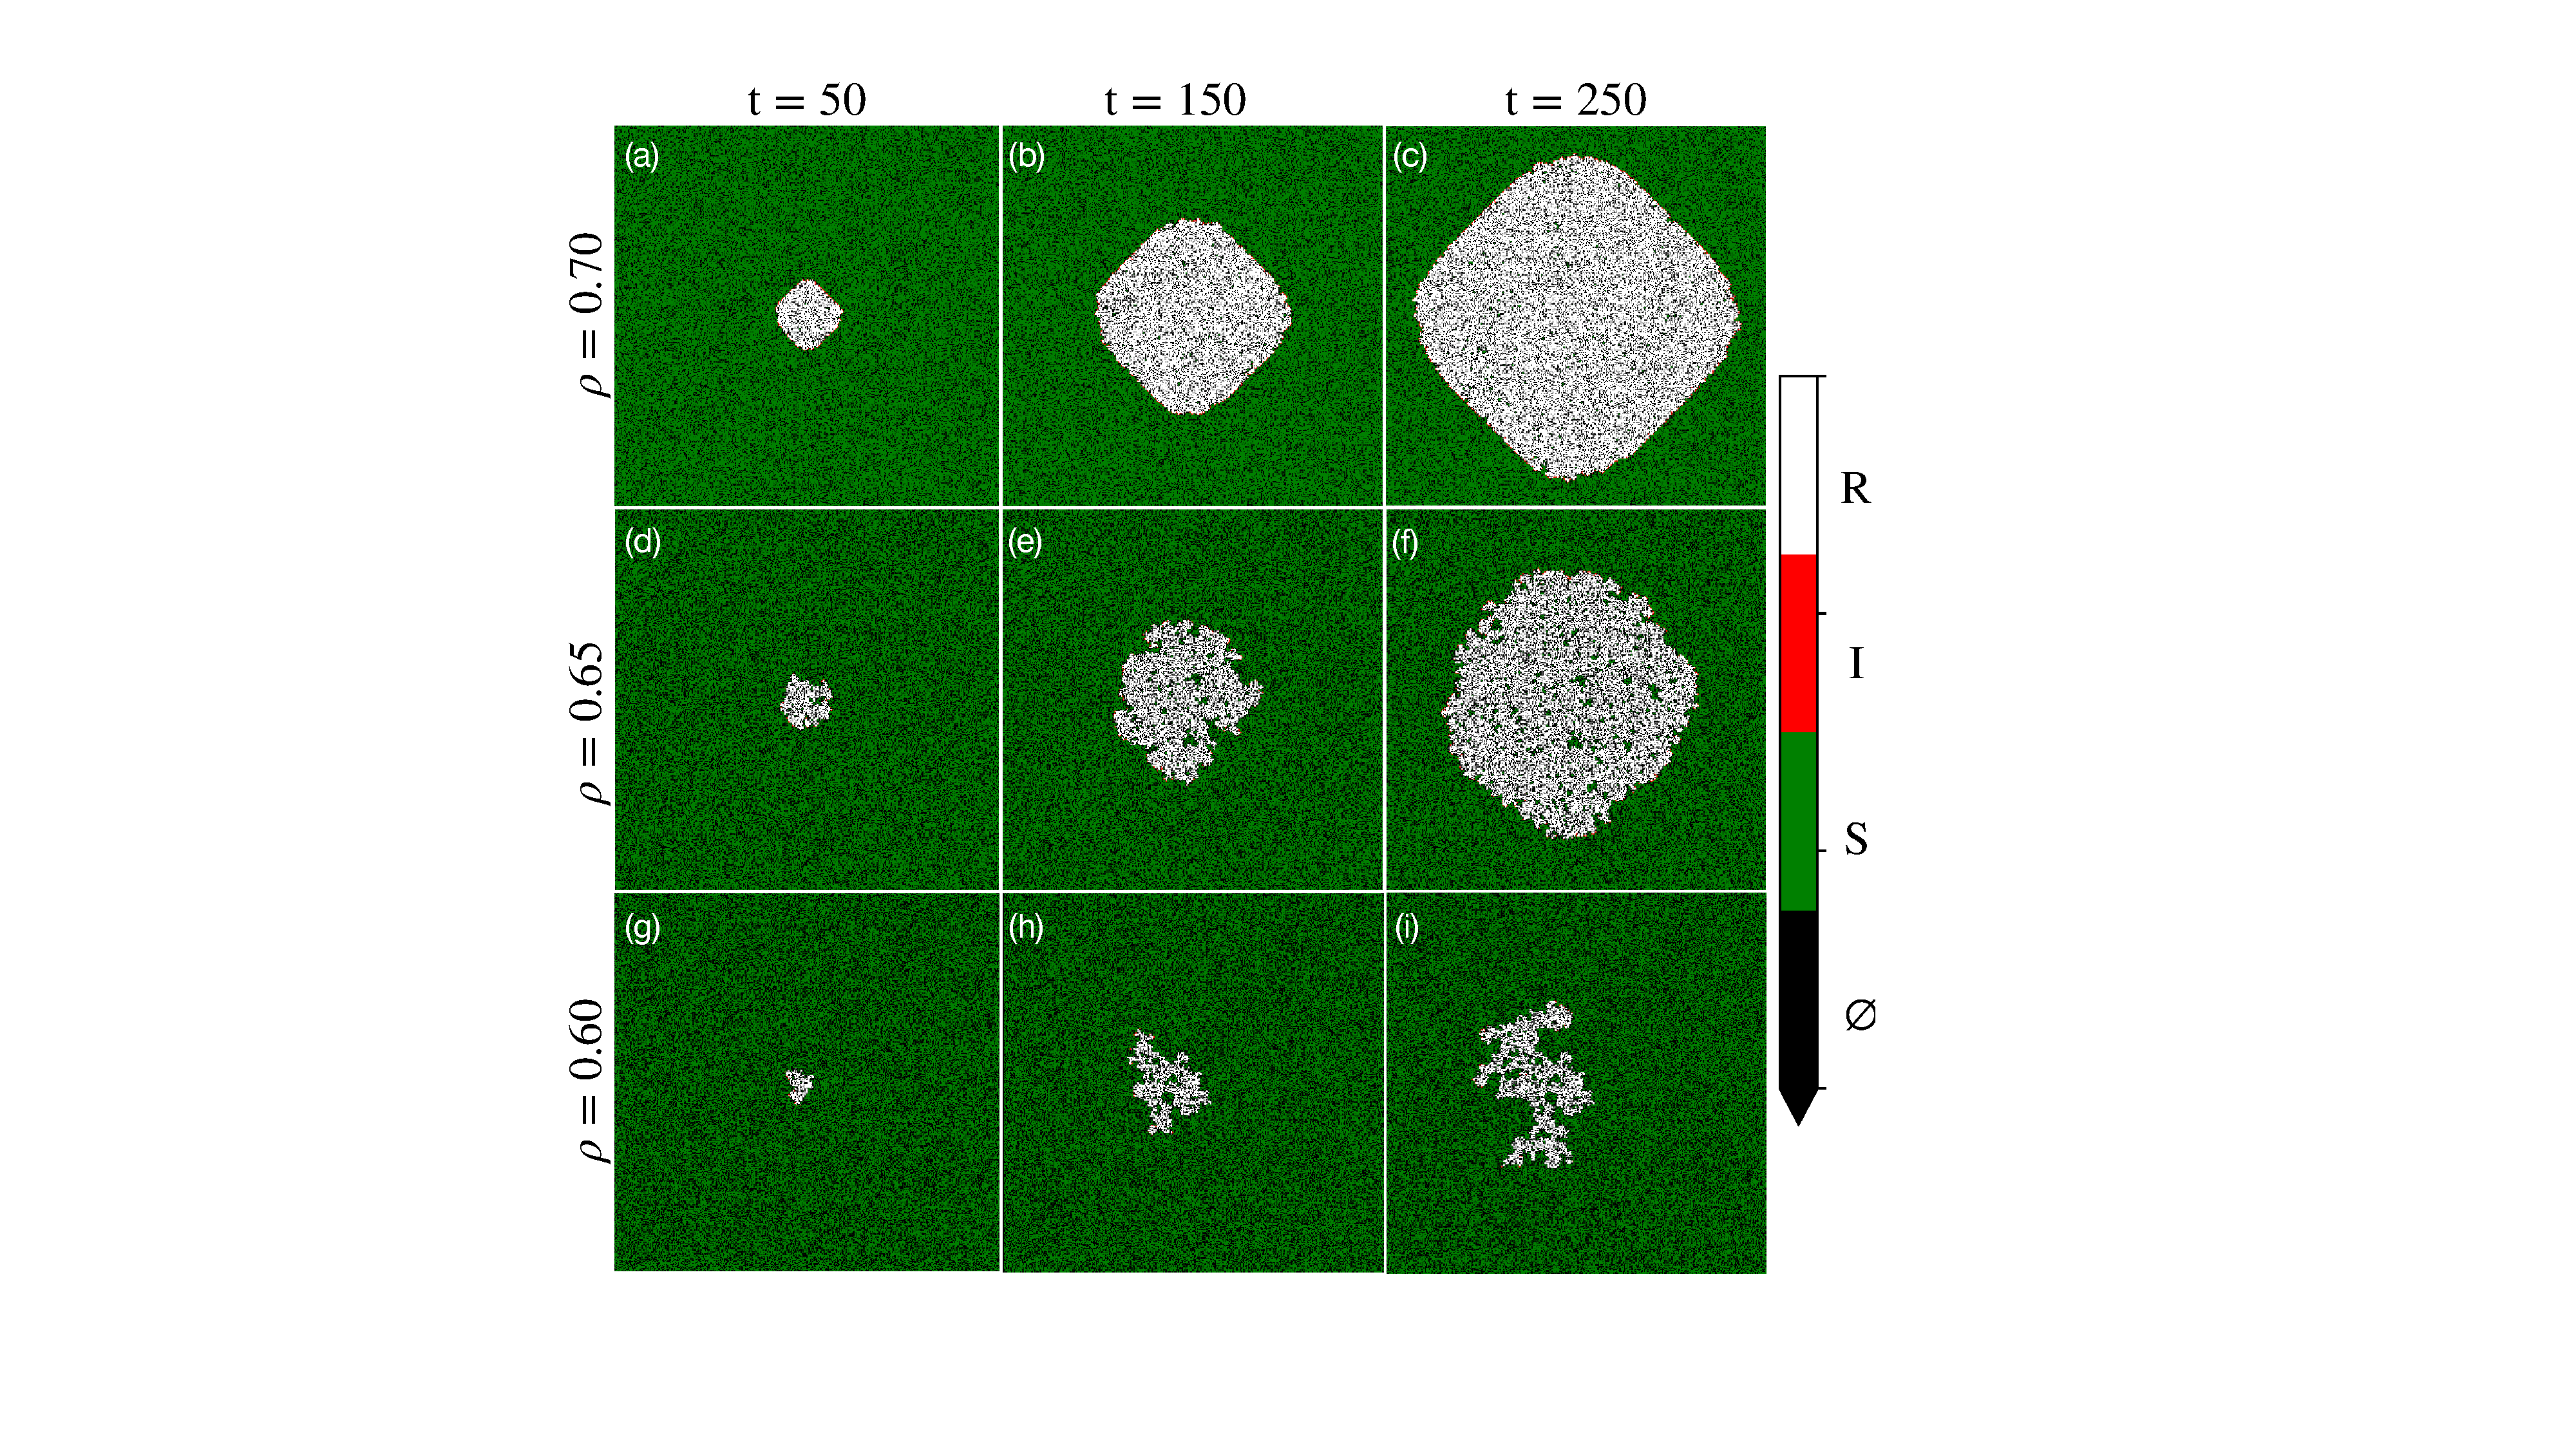
\includegraphics[scale=0.50]{chapter3/figures/figure1-1param-perc.pdf}
    \caption{
        Evolving outbreaks in the one-parameter, percolation-based $SIR$ model are shown for different tree densities ($\rho$).
        From left to right, three successive time-steps are plotted on a domains of size $500 \times 500$.
        Green and black pixels represent susceptible and insusceptible (empty) host units, respectively, 
        while white and red lattice sites depict removed and infectious hosts. 
        (a-c) High-density simulations reveal an unnatural diamond-shaped spread, undesirably reflecting the underlying lattice geometry.
        (d-f) Simulations above the threshold spread radially outward from the epicentre, defining a connected cluster of infectious-removed trees in the process. (g-i) Around the percolation threshold, the disease spreads slowly and chaotically outward. 
        }
    \label{fig:ch3-perc-spread}
\end{figure}

Figure \ref{fig:ch3-perc-spread} illustrates dynamic simulations of disease spread through a series of $500 \times 500 $ domain. At density $\rho=0.70$, Figures \ref{fig:ch3-perc-spread} (a-c) reveal an unnatural diamond-like pattern of spread reflecting artefacts of the lattice geometry.
The diamond-like spread begins to disappear in Figure \ref{fig:ch3-perc-spread}(d-f), when simulations have density $\rho=0.65$. At this density, a wave-like propagation of infected trees spreads radially from the epicentre outward toward the lattice boundary. Interestingly, these observations can be understood through the lens of stochasticity. At a lower tree density, the probability of spread between neighbours is lower, and the spread is more chaotic, thereby disrupting the highly ordered wavefront shown through panels (a-c) into a circular travelling wavefront.
However, it is worth remarking that an alternate triangular or honeycomb lattice geometry would change the diamond-like pattern altogether.

Figures \ref{fig:ch3-perc-spread}(g-i), show the spread of disease for a lower host density of $\rho = 0.60$.
As the disease spreads outward, a more fractal-like pattern begins to emerge.
Moreover, the disease spreads slowly, as evidenced by the smaller area traced by the infectious-removed trees shown from white to red.
In this regime of spread, `persisting' simulations result from the slowly evolving epidemic as it defines a disordered cluster of infectious-removed hosts.
\newpage

\subsection{Percolation threshold}
\label{section:universality}

Consider a simulation with tree density below the epidemic threshold. In this case, an evolving epidemic is unlikely to percolate to the domain boundary, and the pathogen will become extinct. If the host density increases, we can imagine that epidemics begin percolating to the boundary for some specific value.
Consequently, the probability of percolation was examined over a sweep of density parameters, shown in Figure \ref{fig:ch3-perc}(a).
Unsurprisingly, a threshold-like behaviour is revealed. All the simulations that form Figure \ref{fig:ch3-perc}(a) evolved inside a $500\times 500$ sized domain.
The probability of percolation ($Pr(\rho)$) defines a critical region, highlighted in orange (where $ \rho \in [0.57, 0.62$]), that separates regimes of pathogen extinction and percolation/epidemic. The threshold depicted by Figure \ref{fig:ch3-perc}(a) is consistent with the accepted percolation threshold for a two-dimensional square $\rho_c \approx 0.592$.

The value of $Pr(\rho)$ depends non-trivially on stochasticity, which motivated an ensemble-averaged approach\textemdash 
further reading on the underlying theory of ensemble-averaging can be found in \cite{gibbs1902elementary}.
In Figure \ref{fig:ch3-perc}(a), 100 repeated simulations obtain the probability of percolation. Simulations that percolate to the domain boundary assume the numerical value of one, while pathogen extinction events assume zero; for each value of $\rho$, the average value is computed, thus defining a probability $Pr(\rho)$.

At the critical density, denoted by $\rho_c$, we witness the emergence of some exciting phenomena.
Figures \ref{fig:ch3-perc}(c-d) show a spanning cluster ($C_\infty$) of infectious and removed trees (in white to red respectively) at $\rho_c=0.592$.
The cluster looks remarkably similar at all spatial resolutions, said to be `self-similar' \cite{Kapitulnik_1983}.
Within $C_\infty$, one can identify clusters of untouched susceptible trees (in green) of various sizes, suggesting a distribution of cluster sizes occupy all possible length scales.
In the literature, clusters can be described by a `cluster number' ($n_s$) distribution, where $n_s$ is the number of clusters containing $s$ open/susceptible lattice sites.
Furthermore, around the percolation threshold, there can be significant fluctuations in the size of the clusters formed\footnote{
The related statistical fluctuations analysed by \cite{OROZCOFUENTES201912}
present an effective early warning system for the prediction of forest-based pathosystems\textemdash revisited in the next Chapter.
}.

\begin{figure}
    \centering
    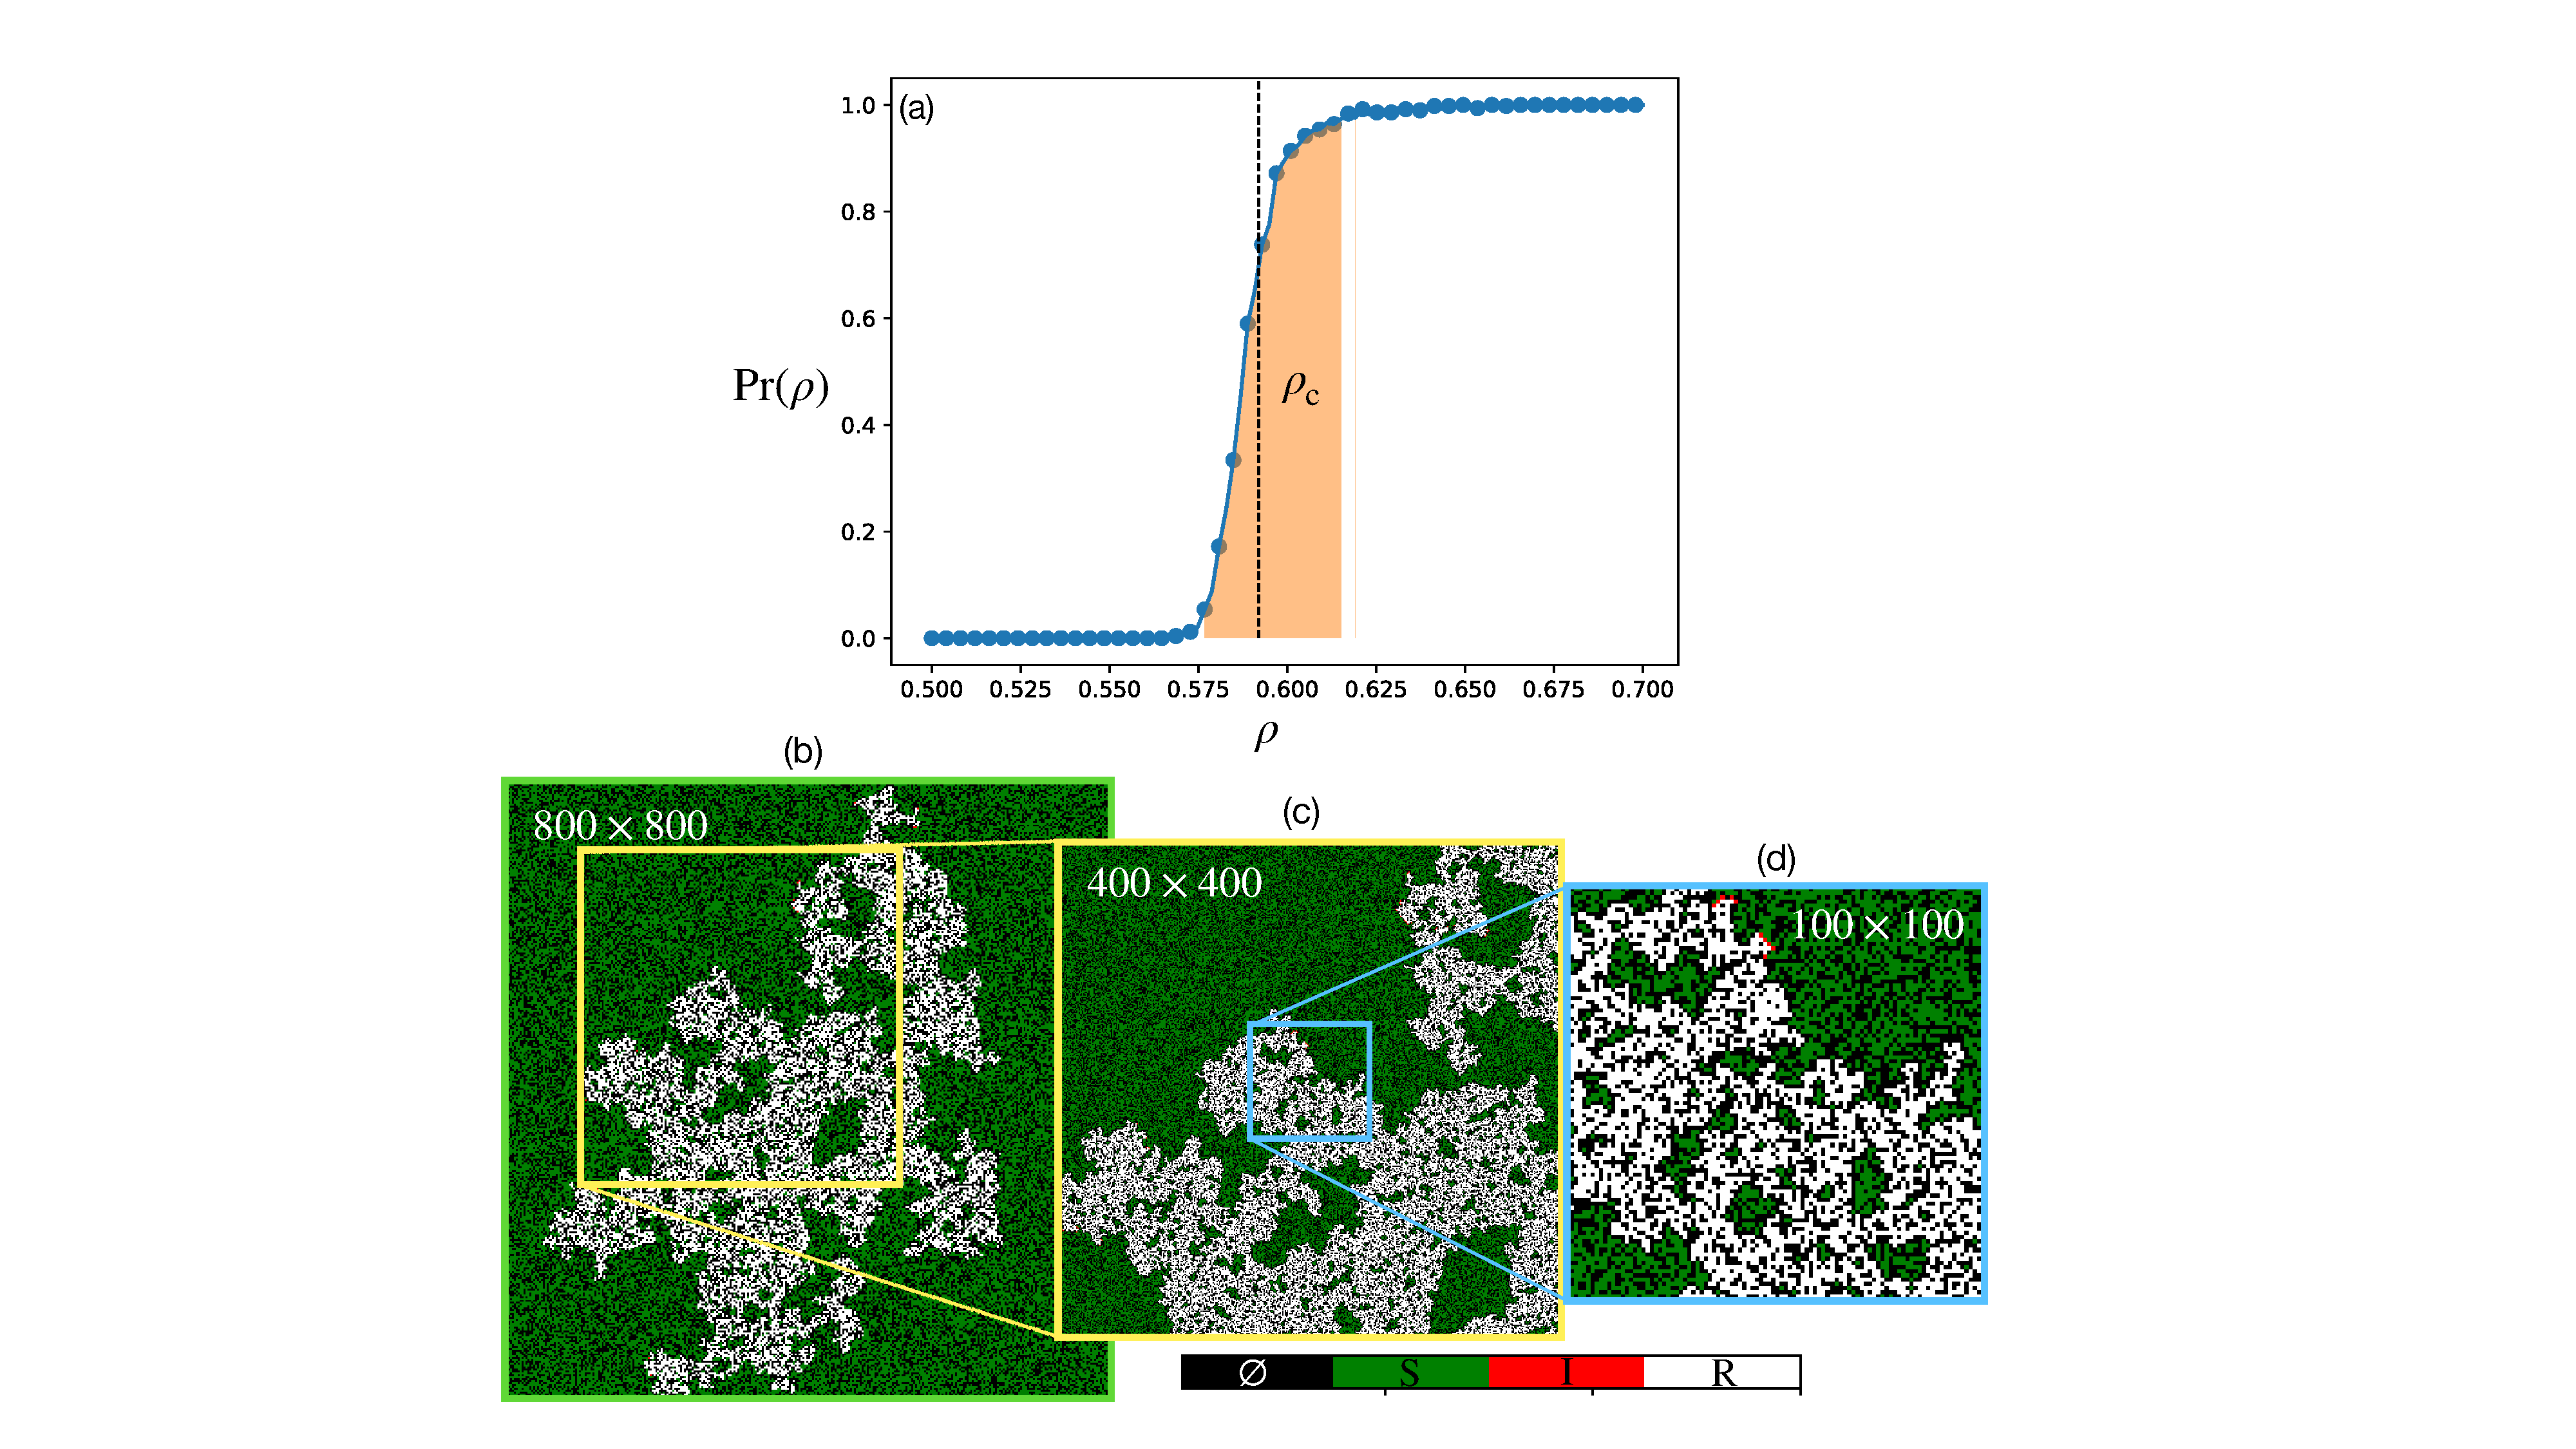
\includegraphics[scale=0.4]{chapter3/figures/figure2-1param-perc-threshold.pdf}
    \caption{The percolation threshold is determined for the one-parameter percolation $SIR$ model.
            (a) The probability of percolation ($\mathrm{Pr(\rho)}$) is plotted against host density.
            The shaped orange region highlights a threshold consistent with results from classical percolation theory, 
            namely $\rho_c = 0.592$, shown by the vertical dashed line. 
            (b-c) At the critical density $\rho_c$, a cluster spanning the domain in (b) is assessed over progressively smaller resolutions.
            Similar features are observed on different scales and scale invariance is observed in the model.
            }
    \label{fig:ch3-perc}
\end{figure}

\begin{table}[h!]
  \begin{center}
    \begin{tabular}{l|c|c|r} % <-- Alignments: 1st column left, 2nd middle and 3rd right, with vertical lines in between
    \hline
      \textbf{Lattice} & NN & \textbf{Site percolation} & \textbf{Bond percolation}\\
      \hline
      1D & 2 & 1 & 1\\
      Square 2D & 4 & 0.593 & $1/2$\\
      Triangular 2D & 6 & $1/2$ & 0.347\\
      Honeycomb & 3 & 0.696 & 0.653\\
      Diamond & 4 & 0.43 & 0.388\\
      Voronoi & - & 0.714 & 0.667\\
    \hline
    \end{tabular}
    \caption{The site and bond percolation threshold for various lattice types\textemdash data published by \cite{stauffer2018introduction, PhysRevE.80.041101}.
            Each lattice configuration defines a set of nearest neighbours (NN).
    }
    \label{tab:perc}
  \end{center}
\end{table}

This Chapter rests on a simulations developed on a square lattice, though we could have considered different configurations, e.g. a triangular, honeycomb or Voronoi lattice.
From the observation of Figures \ref{fig:ch3-perc-spread}(a-c), high host densities would produce highly ordered wavefronts reflecting the different lattice configurations.
In addition, various quantities within the model would change, especially the critical density $\rho_c$ that changes in response to the nearest neighbour (NN) number.
For completeness, table \ref{tab:perc} shows a selection of site and bond percolation thresholds.
Even though $\rho_c$ would change between lattice configurations, some universal properties of the model would remain fixed, 
which leads to a description of universality below.

\subsection{Universality}

At $\rho \sim \rho_c$, percolation and scaling theory explain how the system follows a power law of the form $\propto (\rho - \rho_c)^{\alpha}$ 
where $\alpha$ is a universal critical exponent.
All systems that possess the same exponent are members of the same `universality class' \cite{PhysRev.180.594, RevModPhys.76.663}.
Consider the probability that one open site (at the origin) is connected to another open site a distance $r$ away. 
In this scenario, the probability is described by the `correlation function' $g(r)$. 
The behaviour of this function defines a length scale, denoted as the `correlation length' $\xi$ that dictates how the probability of `connectedness' decays with distance $r$. 
For densities close to percolation threshold: 
\begin{equation}
    \xi \sim |\rho - \rho_c|^{-\nu}
    \label{eq:universal-scaling}
\end{equation}
where $\nu$ is a critical exponent that is universal for all lattice configurations and only depends on the dimension of the lattice used. In general, there are critical exponents for other quantities, e.g. cluster sizes\textemdash discussed more below. 
However, all follow similar power laws, as shown by \cite{stauffer2018introduction, STAUFFER19791}.

Equation \ref{eq:universal-scaling} can be understood by exploring how the connectivity of open sites depend on the density and the divergence that occurs at the threshold $\rho=\rho_c$. 
For low densities, $\xi$ is small because all clusters exist in singlets/triplets.
However, as $\rho$ increases, the mean cluster length increases as more sites become open and connect to form larger clusters. 
As we approach the critical density (from the direction $\rho \rightarrow \rho_c^{-}$) the spanning cluster is formed and $\xi$ diverges towards infinity, $\xi \rightarrow \infty$. 
If one neglects the divergent spanning cluster, a similar picture is painted for densities just above criticality $\rho > \rho_c$. 
That is, the correlation length $\xi$ decays rapidly as $|\rho - \rho_c|$ increases. 
This time however,  mid-to-large sized clusters get absorbed by $C_\infty$ as the density increases;
thus leaving only small untouched clusters, as $\rho \rightarrow 1$ and $\xi \rightarrow 0 $. 
See \cite{STAUFFER19791} for a detailed breakdown of power laws and correlation length.

Lastly, it is worth discussing well-known results on how the cluster sizes (or masses) scale with the lattice dimension. 
If $\rho > \rho_c$, the largest cluster present (denoted by $M$) would scale according to $M\propto L^{2}$. 
In contrast, if $\rho = \rho_c$, $M$ would follow $M\propto L^{1.9}$, 
where $d_F=1.9$ describes the cluster fractal dimension.
If we normalise the cluster by the size of the lattice ($L^2$), the mean density of $M$ will decay as the lattice size increases, i.e. $L^{1.9}/L^2 = L^{-0.10}$. 
Broadly, the critical phenomena found in percolation theory, thermodynamics and magnetism have close ties and are described by similar power laws underpinned by scaling theory \cite{Essam_1980}.


\section{Pathogen infectivity}
\label{ch3:two-param-model}

We have established a percolation-based model of tree disease described by a one-dimensional parameter-space over tree density $\rho$. %
We now extend the parameter-space to include an `infectivity' parameter, denoted by $\beta$. %
Previously, we made an implicit assumption about pathogen transmission. Namely, that infected trees will transmit the infection to susceptible nearest neighbours with perfect fidelity, that is, a probability of $1$. 
In reality, a pathogen may display a range of virulence depending on the environmental suitability or host susceptibility. For example, the fungus \textit{H. fraxineus} causes more severe ash dieback in natural forest ecosystems \cite{marciulyniene2017can} and releases more spores conditional on temperature \cite{chandelier2014detection}.

Here, the parameter $\beta$ is introduced to model infectivity. Now the probability of a susceptible tree becoming infected during a single time-step is given by: $Pr(S \rightarrow I) = \beta$. Appendix \ref{a:propagation} contains more descriptive information on the computational implementation. 
The infectivity parameter describes a transmission `rate' (i.e. per time-step) and is closely linked to the infectious lifetime $T$ of the tree. %
If a susceptible host falls within a von Neuman neighbourhood of an infected host, it will remain susceptible with probability:
\begin{equation}
\label{eq:pr_s_s}
    Pr(S \rightarrow S) = \rho(1 -\beta)^T
\end{equation}
where $T$ is the number of an infectious lifetime. As $T$ increases, the likelihood of a tree remaining susceptible decreases.
Equation (\ref{eq:pr_s_s}) sets the scene for a predictive mean-field theory.
Subsequently, appendix \ref{a:slm-mean-field-theory} outlines steps toward a novel continuum model of tree disease.

Previously in the one-parameter $SIR$ variant, the infectious lifetime played a minor role in determining wavefront because pathogen transmission occurs with a probability of one.
However, now a susceptible host will survive for $t=T$ time-steps before transitioning into $R$. Ultimately, the model is non-dimensionalised, and the value of $T$ is arbitrary. However, a single step can be envisioned to be on the order of years. At this stage, we have recovered the two-parameter model used by \cite{OROZCOFUENTES201912}, which henceforth is referred to as the `\textit{simple lattice model'} (SLM). 

Figure \ref{fig:slm} show three SLM simulations, spreading for the shown infectivity parameters through different time-steps.
All simulations in Figure \ref{fig:slm} are governed by a fixed value of $T=10$, and density $\rho=0.70$.
The colour bar in Figure \ref{fig:slm} represents different steps through the infectious period, from yellow to red.
Higher values of $\beta$ yield a faster spreading velocity,
as expected.
Figures \ref{fig:slm}(g-i) allude to $\beta$ altering the percolation threshold, on the basis of $\beta=0.25$ reflecting a more fractal-like spreading pattern, even well beyond the standard percolation threshold of $\rho_c=0.592$.

Figure \ref{fig:slm-wave-front} shows how variations in the infection lifetime can change the wave-front properties. 
The value of $\beta$ predominantly controls the speed of the wave-front, whereas $T$ controls the lag-time on the removal front. 
Therefore, increasing $T$ yields an increase in the wave-front thickness;
this is valid for $\rho > \rho_c$.
Around the percolation threshold $\rho \sim \rho_c$, the relationship between $T$ and spreading velocity is less obvious. 
Close to the percolation threshold, variations in $T$ have more importance, as it could lower or raise pathogen transmission below or above percolation thresholds, respectively.
If $T$ is held fixed, the critical threshold definition can now be generalised from Equation (\ref{eq:critical_threshold_1d}), to include the parameter $\beta$: 

\begin{equation}
\label{eq:critical_threshold_1d}
    \rho _{c}=sup \lbrace \rho, \beta : \theta (\rho, \beta ) = 0 \rbrace
\end{equation}

\begin{figure}
    \centering
    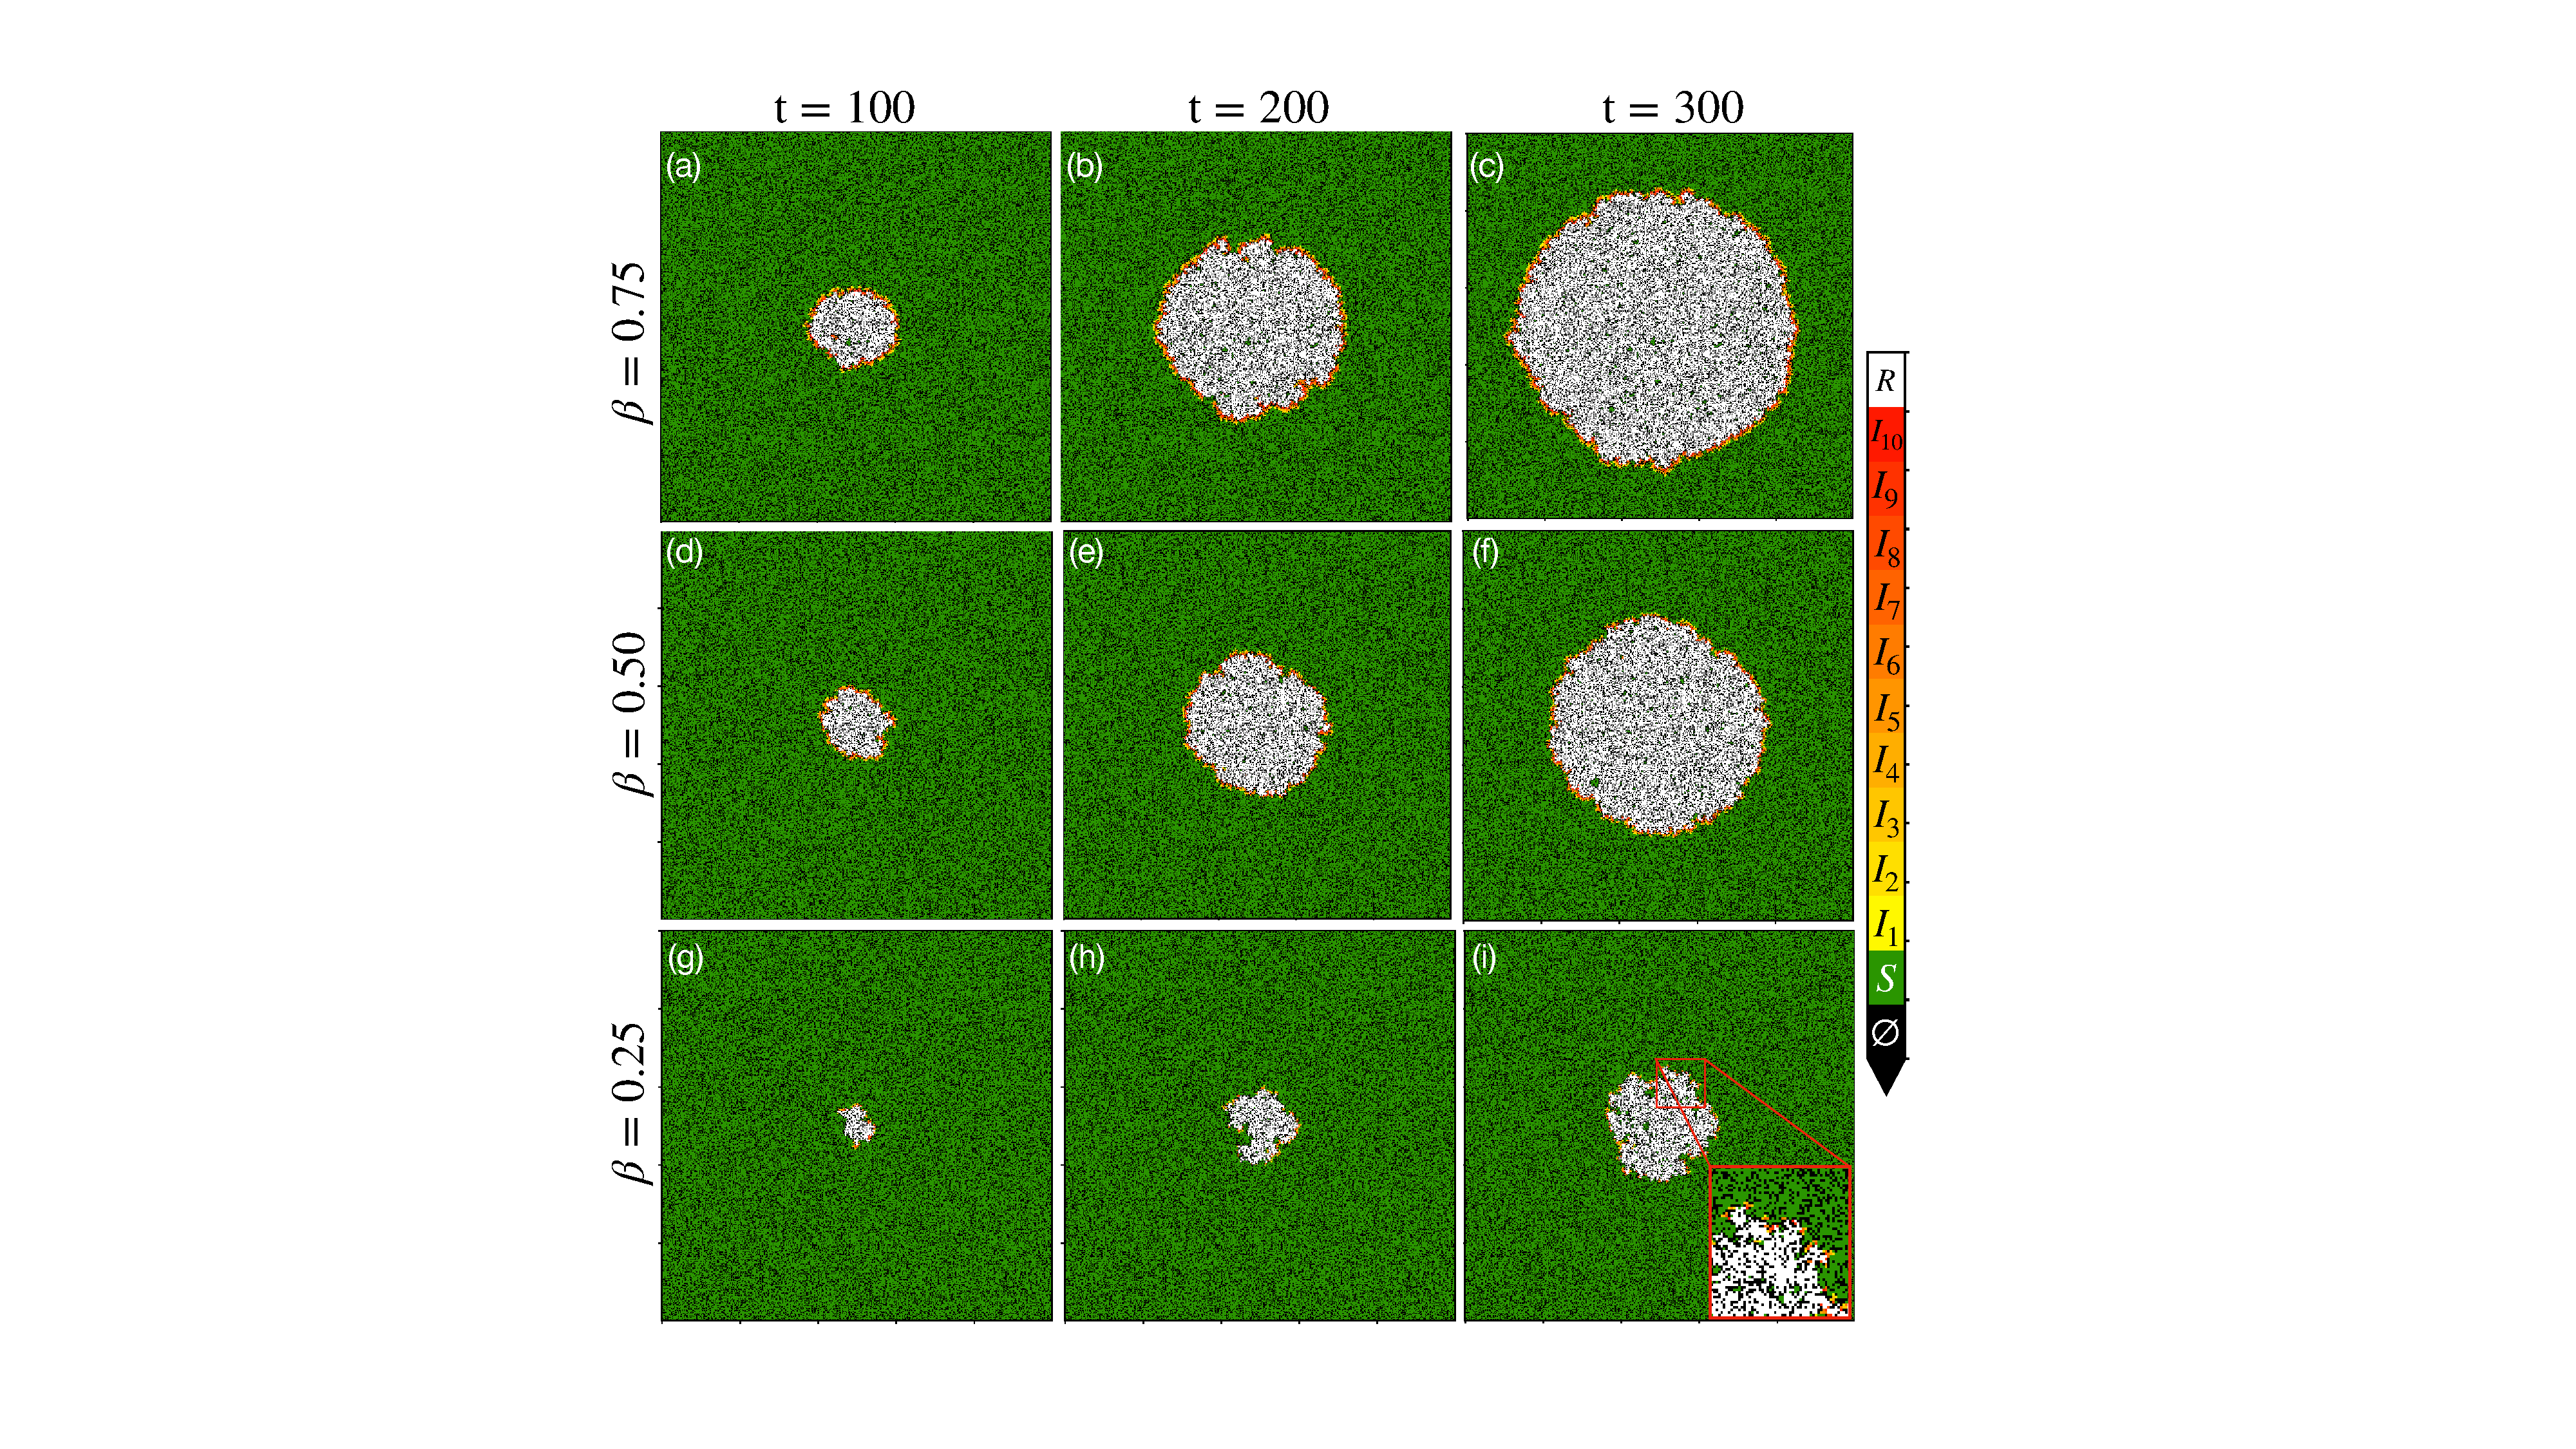
\includegraphics[scale=0.45]{chapter3/figures/figure3-two-param-model.pdf}
    \caption{Introducing an infectivity parameter $\beta$. The SLM is shown running on a domain of size $500\times500$ for fixed $T=10$ and density $\rho=0.70$. Simulation reveal that $\beta$ has an impact on the wave-front speed and changes the percolation threshold.}
    \label{fig:slm}
\end{figure}

\begin{figure}
    \centering
    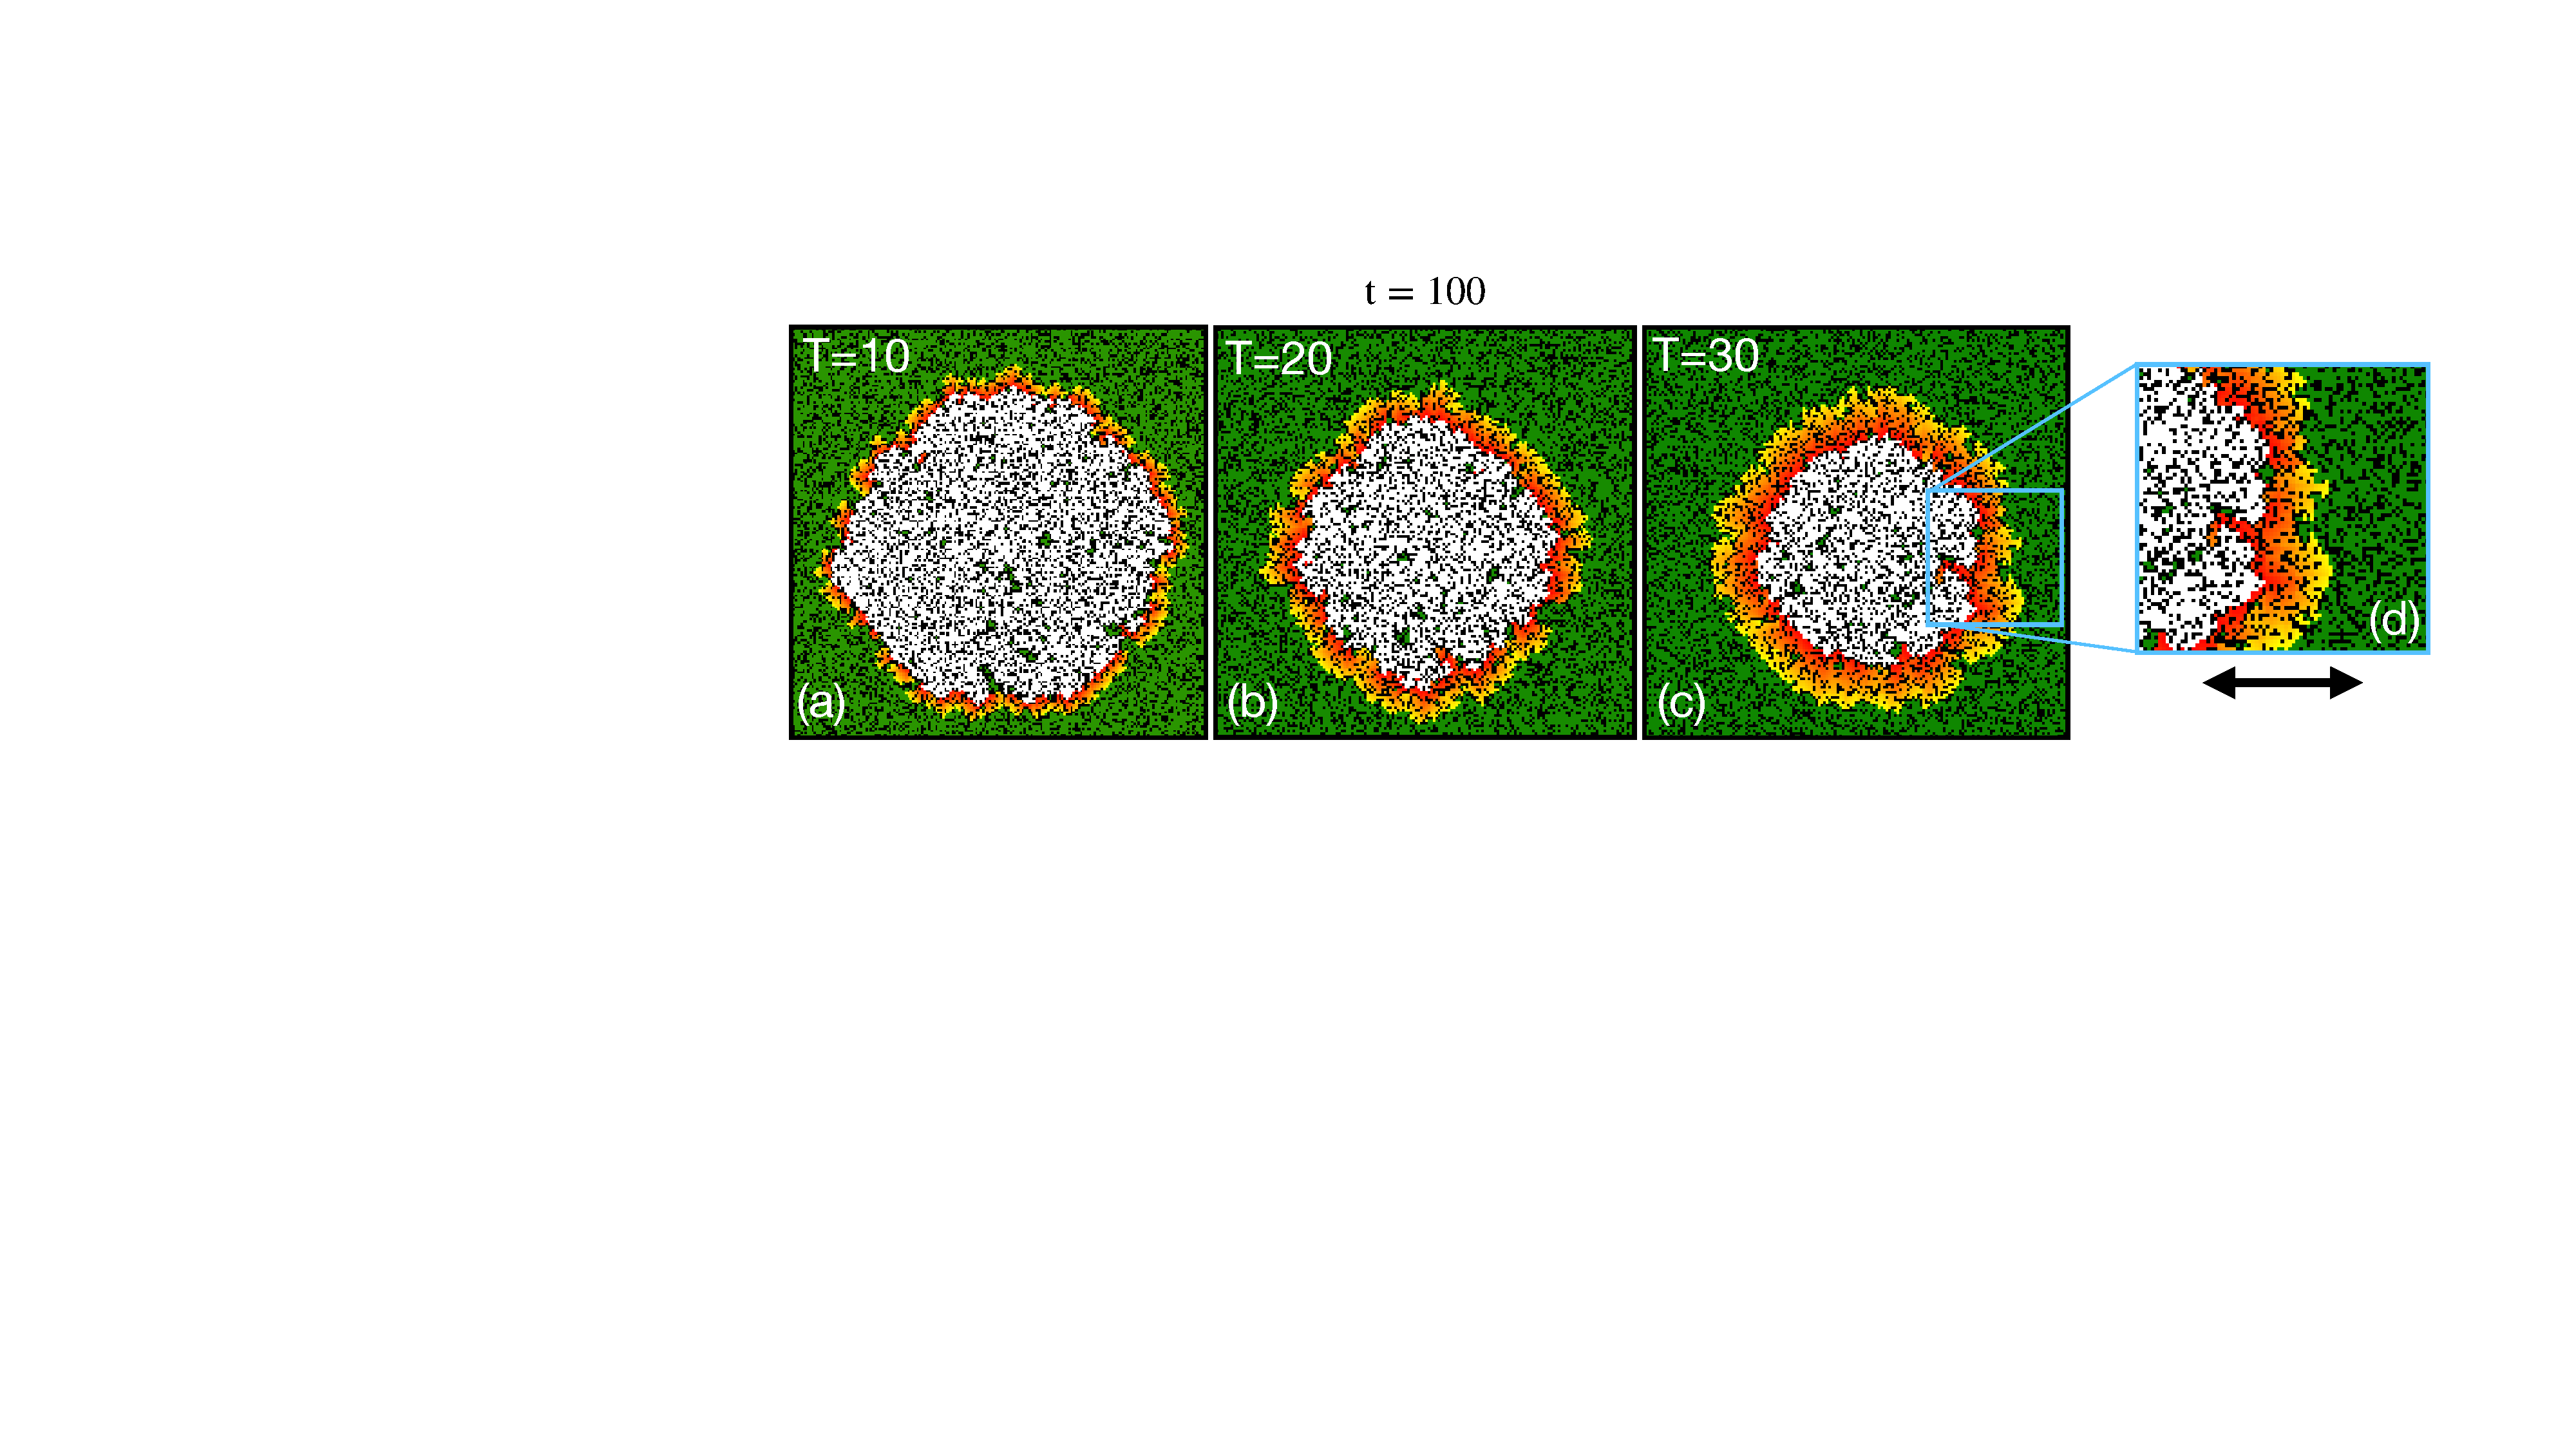
\includegraphics[scale=0.35]{chapter3/figures/figure5_.pdf}
    \caption{Simulations with varying infectious lifetimes $T$, shown through the time-step $t=100$.
    For fixed $\rho$ and $\beta$ above the threshold, varying $T$ has no impact on the speed of the wavefront. 
    However, increasing $T$ leads to a thicker wavefront, as the posterior interface (between $R$ and $I$) lags behind the evolving wave-front (between $S$ and $I$).}
    \label{fig:slm-wave-front}
\end{figure}

\newpage

\section{Epidemic thresholds}
\label{sec:SLM-epidemic-threshold}

Previously in section \ref{section:universality}, the percolation probability was examined over one parameter of host density.
A threshold occurred over a narrow range of densities and separated the regime of epidemic and pathogen extinction.
Notwithstanding, we did not examine the rate of pathogen propagation nor any additional dynamic information.
In order to capture spreading rates, a metric comprising the `spreading velocity' is introduced, captured by: 
\begin{equation}
\label{eq:vel_eff_r}
    v_{radial(t)}=\sqrt{N_I(t+1)-N_I(t)}
\end{equation} 
where, $N_I$ is the number of infected trees in the domain at time-step $t$. 
The difference in $N_I$ between time-steps gives an `effective' radial velocity. %
The number of spatial units progressed by the pathogen is averaged over all angles per unit time. %
Strictly speaking, Equation (\ref{eq:vel_eff_r}) is valid only for $\rho > \rho_c$. At the percolation threshold, the wave-front assumes a fractal dimension and averaging over two dimensions becomes unreasonable.

The time-series, $v_{radial}(t)$ is shown in Figure \ref{fig:vel_eff_rad_metric}(a) for three combinations of $(\rho, \beta)$.
Unsurprisingly, higher-valued combinations produce a higher velocity.
Additionally, initial instability is most significant through the first $\sim 200$ time-steps, a consequence of the initial conditions which suggests the system has yet to reach a steady state.
Here, the system is said to be in a transient state.
In Figure \ref{fig:vel_eff_rad_metric}(a), a simulation average $\overline{v}_{radial}(t)$, 
can be determined and plotted as a horizontal line, repeating the measurement multiple times over an `ensemble', gives a probability distribution. 

Figures \ref{fig:vel_eff_rad_metric}(b-d) display the probability density functions\footnote{
To reduce artefacts of initial transience, any simulation that became extinct before the initial transient period 
of $t_{tr}\approx 200$, was excluded from calculations of the ensemble mean.} of the mean velocities.
In all panels, the vertical black line inside each distribution depicts the ensemble mean velocity.
For higher host densities, the mean velocity increases and distributions appear somewhat narrower.
Additionally, Figures \ref{fig:vel_eff_rad_metric}(b-d) suggest that $\beta$ plays a role in determining the velocity variance, as the distributions become wider with lower infectivity, cf. the green and blue distributions.

For now, the important statistic is merely the ensemble mean, denoted by $\big\langle\overline{v}\big\rangle$.
although, from Figures \ref{fig:vel_eff_rad_metric}(b-d), we can begin to access the third-order statistical moment of skew.
Namely, the green distributions become progressively right-skewed as density is lowered.
Statistical measures over the ensemble have exciting applications and can detect an early warning signal, a topic covered in the next Chapter.

\begin{figure}
    \centering
    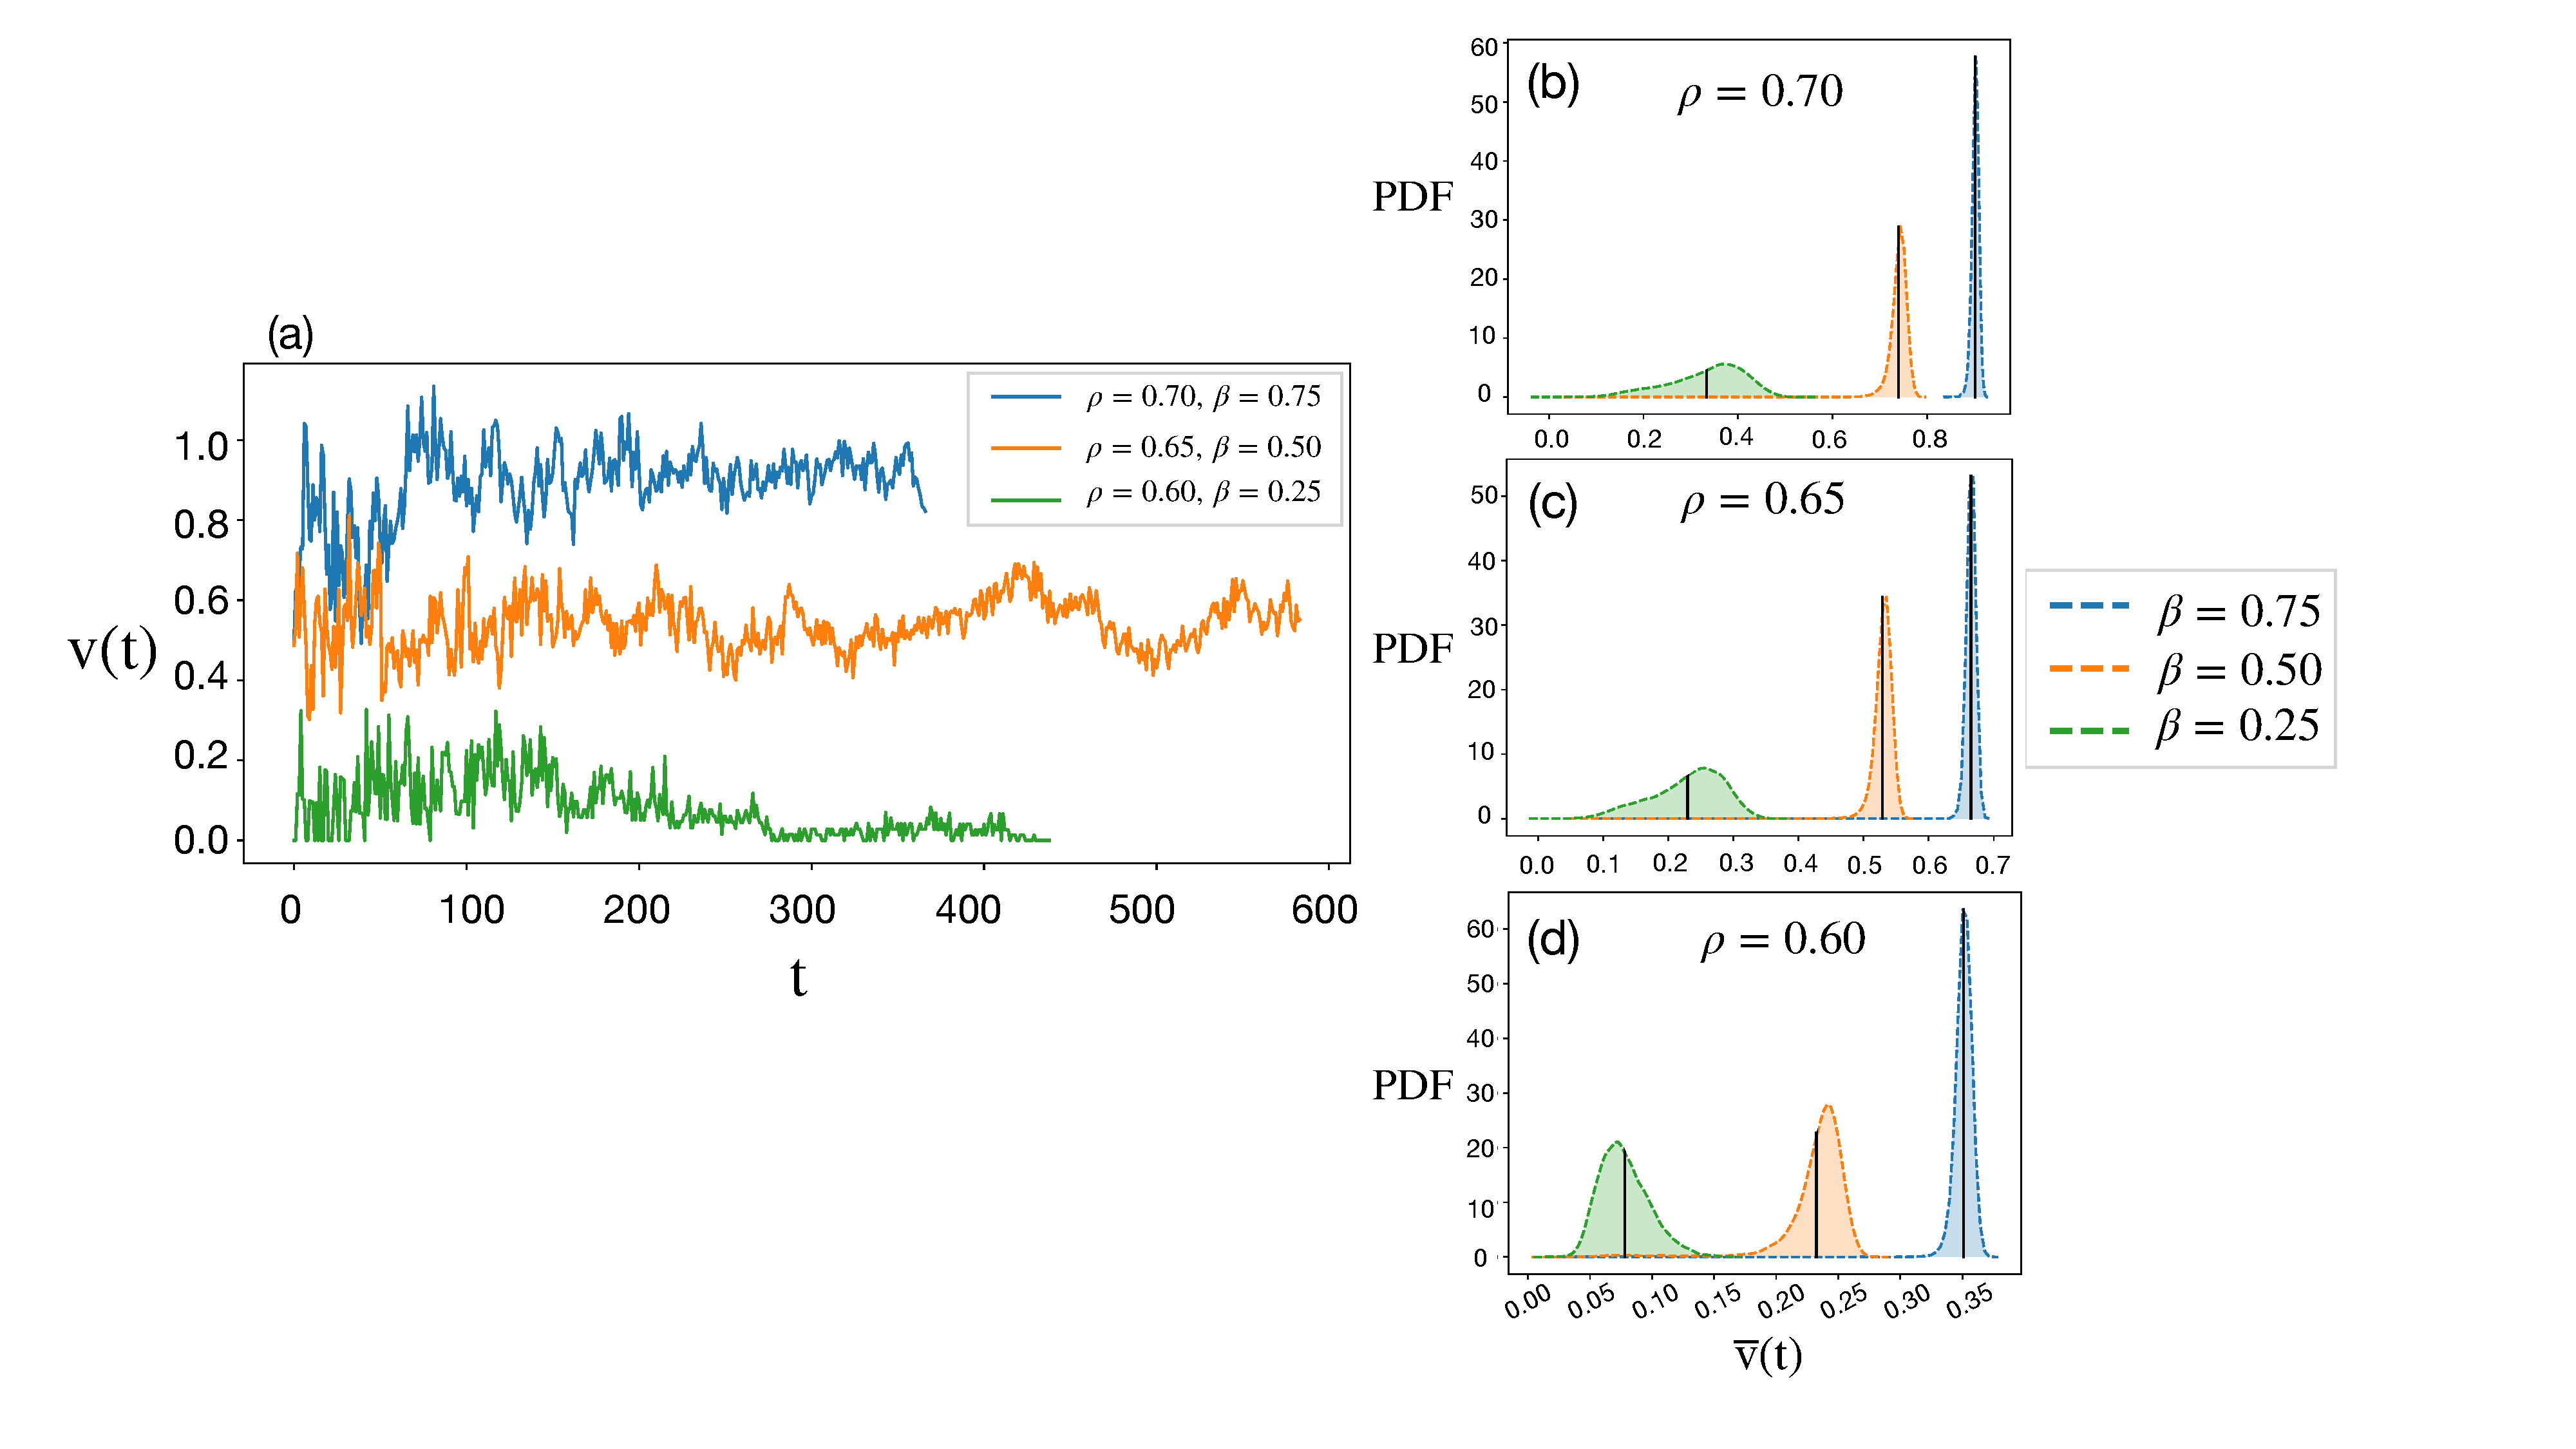
\includegraphics[scale=0.26]{chapter3/figures/figure7.pdf}
    \caption{(a) The velocity metric time-series $v_{radial}(t)$ is shown for three typical simulations, higher values of $\rho$ and $\beta$ give higher mean values of propagation speed. (b-d) The probability density function of mean spreading velocity $\big\langle \overline{v}_{radial}(t) \big\rangle$ for variations in $\rho$ and $\beta$.}
    \label{fig:vel_eff_rad_metric}
\end{figure}

Figure \ref{fig:slm_pspace} contrasts the epidemic threshold according to both percolation and velocity-based metrics.
In Figure \ref{fig:slm_pspace}(a), a one-dimensional line through the parameter-space of $\rho$ reveals the percolation probability for the three different infectivity parameters shown.
The vertical dashed line shows the accepted percolation threshold, $\rho_c$, for a two-dimensional square lattice. 
For $\beta \in [0.50, 0.75]$, the probability of percolation is identical to that shown in Figure \ref{fig:ch3-perc};
However, a lower value of $\beta = 0.25$ decreases the percolation threshold, as evidenced by the green line shifting to the right.
Figure \ref{fig:ch3-perc}(a) intuitively demonstrates that a pathogen with a low value of infectivity requires a more significant tree density to spread.

The ensemble-averaged radial velocity $\big\langle \overline{v} \big\rangle$ (as per Equation \ref{eq:vel_eff_r}) mirrors the percolation threshold,
notwithstanding with some differences.
In Figure \ref{fig:slm_pspace}(b), we witness a significant increase in the propagation speed when the density crosses the threshold density $\rho_c$, 
notably for $\beta=0.75$ and $\beta=0.50$ shown in blue and orange. 
In addition, a higher $\beta$-value predictably yields a higher radial velocity, both before and after the epidemic transition.

The green curve ($\beta=0.25$) in Figure \ref{fig:slm_pspace}(b) alludes to an important regime in the model.
Namely, a regime of `persistence' \cite{gilligan2008epidemiological}.
The vertical dashed green line highlight when epidemics begin to propagate to the domain edge reliably ($95\%$ percolation).
Thus, the chance of percolation in Figures \ref{fig:slm_pspace}(b) is high, yet the velocity remains close to zero.
Together, these observations reveal a region in parameter space where epidemics can survive for long periods, barely above the threshold.
Nonetheless, host population growth is omitted from the model so persistence is only approximate.

The equivalent two-dimensional plots over the full parameter-space of $\rho$ and $\beta$ are shown in Figures \ref{fig:slm_pspace}(c-d) for percolation and radial-velocity, respectively. 
Percolation in Figure \ref{fig:slm_pspace}(c) reveals an abrupt transition between two stable regimes of extinction and epidemic, separated by a narrow range of critical parameters $\rho_c$ and $\beta_c$.
In Figure \ref{fig:slm_pspace}(d), the ensemble-averaged velocity reveals a smoother transition between states.
As the distinction between epidemic states is more apparent in Figure \ref{fig:slm_pspace}(c), one might argue that percolation captures the threshold with greater clarity.
When infectivity is lower ($0.15 <\beta<0.30$), the percolation threshold can be crossed by raising the density, reflected in both velocity and percolation metrics.
However, percolation has no dependence on infectivity beyond $\beta \approx 0.40$, in contrast to the radial velocity that tends to increase for higher infectivities, revealing a subtle difference between metrics.
Here, the parameter-sweeps can be understood to portray an `\textit{epidemic phase diagram}'.

\begin{figure}
    \centering
    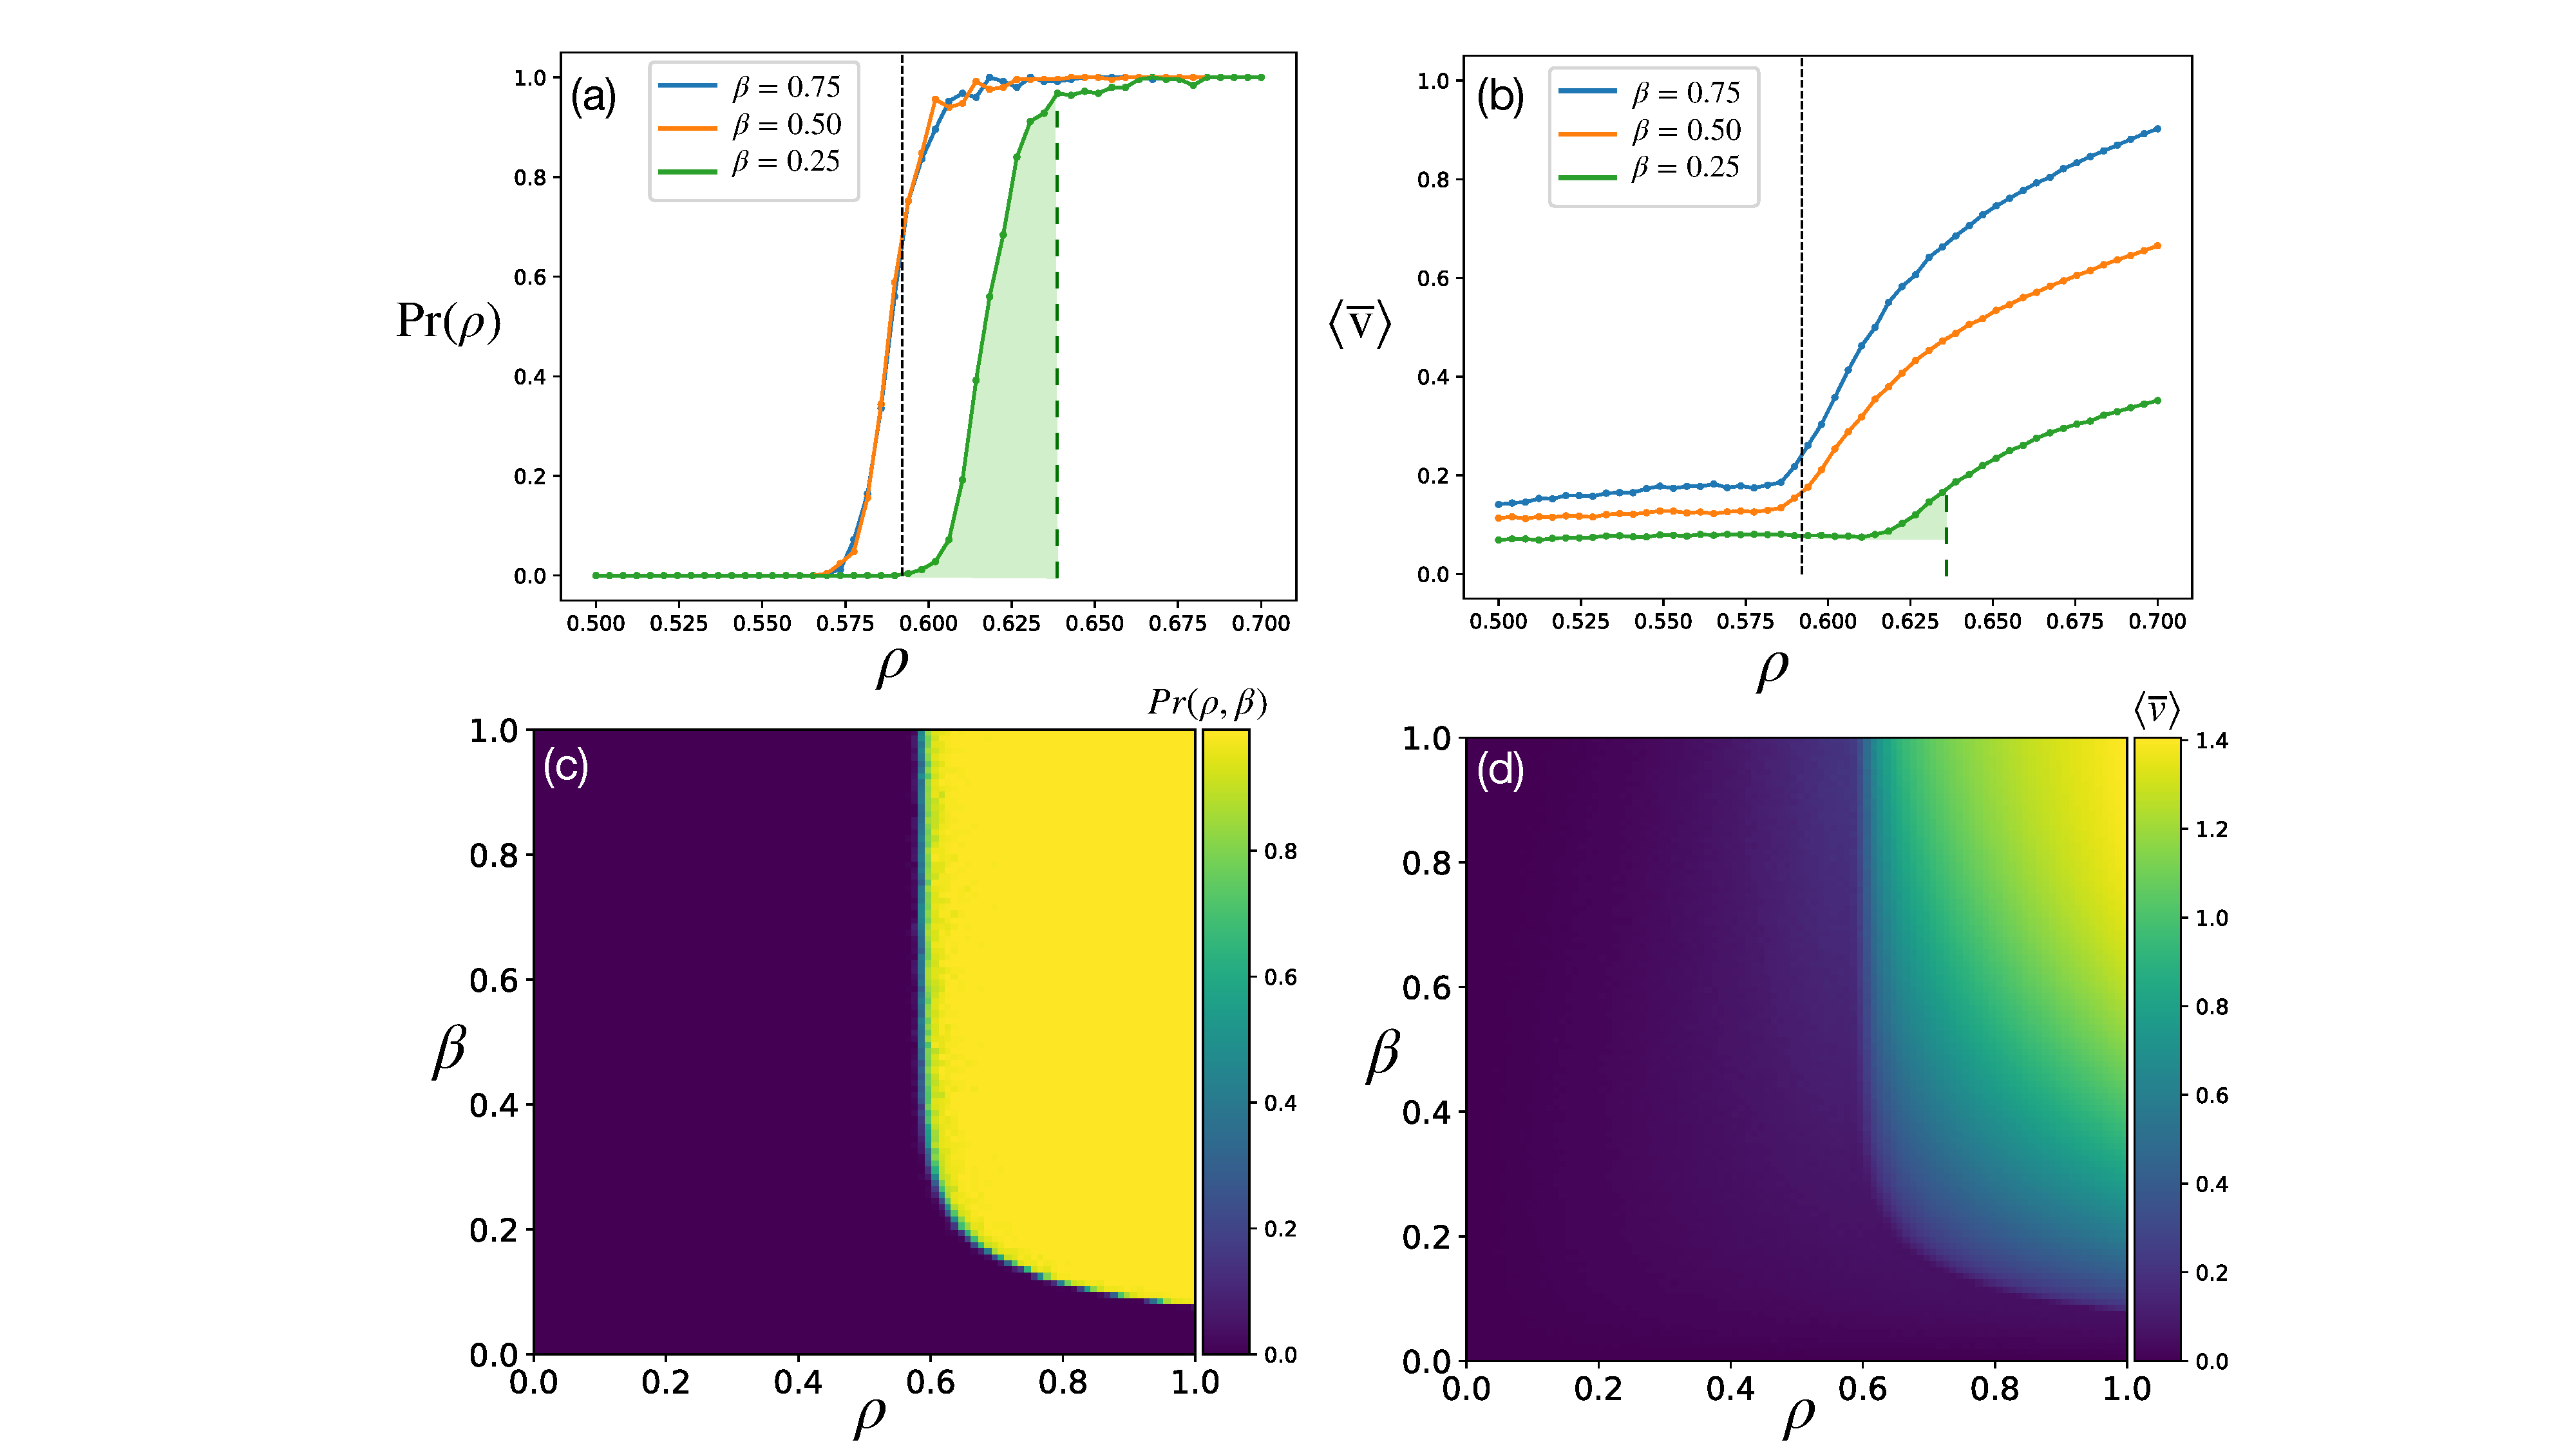
\includegraphics[scale=0.325]{chapter3/figures/figure4-perc-vel-phase-trans.pdf}
    \caption{
    A parameter sweep of $\rho$ and $\beta$ over the $500\times500$ domain. (a-b) The percolation probability is shown alongside the radial velocity over a one-dimensional parameter-space of $\rho$. For the lower-valued infectivity of $\beta=0.25$, the density threshold is slightly higher than classical percolation  $\rho_c=0.592$, indicated by the vertical dashed line. A gradual increase occurs when using the radial velocity, whereas percolation shows an abrupt transition. (c-d) A two-dimensional parameter sweep paints a similar picture.
    }
    \label{fig:slm_pspace}
\end{figure}

\newpage

\section{Discussion}

This Chapter introduced percolation theory, leading to a one-parameter percolation $SIR$ model of tree disease spreading through a forest.
The one-parameter model exhibited stochasticity on account of the randomly populated host distribution inside a square lattice. 
Assessing the model on one lattice configuration signifies a limitation in our analysis, and a comprehensive treatment might consider examining the spread of disease on alternate lattices, e.g. the triangular, honeycomb or Voronoi lattice. Nevertheless, although we examined behaviour on one lattice type, the universal properties of the model would remain fixed. For example, the critical exponent describing the correlation length $\xi$\textemdash as discussed in section \ref{section:universality}.

In section \ref{ch3:two-param-model}, an infectivity parameter ($\beta$) was included in the model.
The infectivity parameter introduced temporal stochasticity into the system, as infections spread probabilistically between nearest neighbours\textemdash as opposed to the one-parameter model that spreads between hosts with a probability of one.
The infectivity parameter altered the critical density; 
higher values of $\beta$ recovered the standard percolation threshold for a two-dimensional square lattice ($\rho_c\approx 0.592$), 
while lower values of $\beta$ increased the critical density required to support an epidemic.

In nature, a pathogen might interact with diverse hosts over numerous environmental conditions.
A relevant and interesting example includes the algae-like oomycete \textit{Phytophthora ramorum} (\textit{P. ramorum}). 
The pathogen \textit{P. ramorum} affects a wide host range \cite{GRUNWALD2012131}, 
including Larches (deciduous conifers of the genus \textit{Larix}) and southern beech (\textit{Nothofagus}), 
and some non-native oaks such as red oak (\textit{Quercus rubra}) \cite{grunwald2008phytophthora}.
Moreover, different genetic variants of \textit{P. ramorum} affect different hosts with varying severities.
For example, North American oak species appear more susceptible to the NA1 lineage \cite{rizzo2002phytophthora},  while UK larch trees appear slightly more highly susceptible to the European lineage EU1 \cite{king2015planta}. Accordingly, although the integration of $\beta$ in the SLM is undoubtedly simplistic and general, it permits a description of varying degrees of pathogen virulence nonetheless.

Two metrics categorized the model's behaviour: the pathogens average radial velocity and a probability of percolation.
The percolation probability defined a sharper, more reliable transition between epidemic and pathogen extinction.
Conclusively, the percolation probability proves more accurate to classify epidemic regimes.
Nevertheless, the radial velocity captured a similar threshold-like behaviour besides additional dynamic information in the form of a time series.
Subsequently, the time series velocity was ensemble-averaged and examined over a sweep of $\rho$ and $\beta$ values. 

Interestingly, comparing the percolation probability to radial velocity revealed a parameter region above the threshold where the pathogen survives but slowly propagates to the domain boundary.
However, as host population growth is neglected in the SLM, long-term host-pathogen coexistence between is prevented and persistence is merely approximate \cite{gilligan2008epidemiological}. 

As we look to construct a more representative model, it is worth remarking on the most significant assumptions that underpin the SLM so far:
\begin{enumerate}
    \item \textbf{Local NN interactions}: in reality, many dispersal mechanisms exist to propagate the spread of disease\textemdash 
    section \ref{ch2:dispersal} contains more information. 
    Undesirably, local interactions in the SLM revealed unnatural artefacts of lattice geometry, witnessed in Figures \ref{fig:ch3-perc-spread}(a-c).
    Moreover, as the pathogen could not jump over empty lattice sites, epidemics were only possible above the percolation threshold, 
    i.e. when connected clusters of hosts span the domain.  
    
    \item \textbf{Uniform dynamics:} in general, pathogen-host interactions transpire with varying degrees of severity.
    For example, age-dependent severity in ash dieback and the species-level virulence of \textit{P. ramorum}. 
    In contrast, the SLM considers that: (A) the transition probability into $R$ occurs with a uniform number of steps 
    (B) the probability of transition into $I$ is identical between hosts 
    (C) $\beta$ is simplistic, with no spatio-temporal (environmental) dependence. 
    More broadly, we have constructed a general, abstract model with no specific pathogen in mind and uniform, simplistic interactions.
    
    \item \textbf{Host distribution}: natural tree populations present rich spatial structures with varying degrees of clustering and aggregation \cite{doi:10.1086/342823}.
    Indeed population clustering has been confirmed over various spatial, from the tree-level to the field-level \cite{wiegand2007analyzing}.
    Therefore, the flat randomly distributed host population considered in this Chapter falls short of a realistic description.
    In addition, the SLM describes the spread of disease in a densely populated forest.
    Hence, as we look to model the spread of disease over Great Britain, realistic tree canopy cover data should be incorporated into the framework.
\end{enumerate}
Despite the assumptions and simplicity of the SLM, it provides a general setting upon which to elaborate.
The next Chapter outlines all the applications that were investigated using the SLM.
\newpage